\section{Modos de Sincronización de Acciones utilizando Redes de Petri}
\subsection{Petición de ejecución versus Aviso de ejecución.}
\subsubsection{Estudio de la Red de Petri de una cinta transportadora}
En esta sección se hará estudio de un caso de uso donde se pueden analizar
diferentes formas de sincronizar una secuencia de acciones utilizando una red de
Petri.\\

\begin{labeling}{alligator}
\item [Ejemplo]
Cinta transportadora con 3 estaciones. Piezas son depositadas en la primer
estación  de manera asincrónica. Cuando esto sucede, la cinta avanza a la
estación 1, donde un operario realiza una transformación a la pieza. Una vez el
operario realizó la transformación, presiona un pulsador y la cinta avanza a la
estación 2, donde un segundo operario empaqueta la pieza. Este segundo operario
presiona otro pulsador al finalizar su tarea y luego la cinta avanza una vez
más y la pieza cae en un contenedor.
\end{labeling}

\begin{figure}[H]
    \centering
    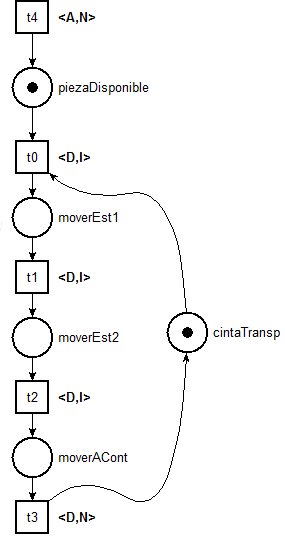
\includegraphics[height=100mm]{Petri_Cinta_Transportadora_1}
    \caption{Red de Petri de una cinta transportadora}
    \label{fig:petri_cinta_transportadora_1}
\end{figure}

\subsubsection{Análisis de ejecución del caso de estudio usando aviso de
ejecución} 
De acuerdo al modo de ejecución por aviso, es el resto del framework el
responsable de dar aviso de eventos al monitor, desencadenando la ejecución de las acciones:
\begin{enumerate}
    \item Debe insertarse un evento en la cola de entrada de “t0” cuando la
    acción escuchando el sensor detecte la llegada de una nueva pieza. Si la
    cinta Transportadora se encuentra disponible, el monitor de petri dispara
    “t0” y se genera un evento que se deposita en la cola de salida de “t0”.
    \item El manejador de eventos lee el evento de salida de “t0” y llama a
    ejecutar la acción “moverEst1”, que mueve la pieza a la estación 1 y espera
    el trabajo del operador. Una vez que el operador realiza su trabajo,
    presiona el pulsador generando un evento que el manejador de eventos, a través del
    mapa de eventos envía a la cola de entrada de “t1”. El monitor de petri
    dispara “t1” y se genera un evento que se deposita en la cola de salida de
    “t1”.
    \item El manejador de eventos lee el evento de salida de “t1” y llama a
    ejecutar la acción “moverEst2”, que mueve la pieza a la estación 2 y espera
    el trabajo del operador. Una vez que el operador realiza su trabajo,
    presiona el pulsador generando un evento que el framework envía a la cola
    de  entrada de “t2”. El monitor de petri dispara “t1” y se genera un evento
    que se deposita en la cola de salida de “t2”.
    \item El manejador de eventos lee el evento de salida de “t2 y llama a
    ejecutar la accion “moverACont”, que mueve la pieza al contenedor. Una vez
    terminada esa acción envía un evento a la cola de entrada de “t3”. El
    monitor de petri dispara “t3” y libera la cinta Transportadora para procesar otra pieza.
\end{enumerate}

Si bien parece prometedor suscribir las tareas a una transición informada (que
avisa al manejador de eventos cuando están dadas las condiciones de ejecución),
tras analizar este modo de sincronización se llega a la conclusión de que existe
una gran desventaja al utilizar la ejecución dirigida por informes. Al utilizar la
suscripción a transiciones informadas el manejador de eventos y manejador de
acciones están asumiendo una parte del rol de control de flujo de ejecución.
Esta responsabilidad debería delegarse por completo al monitor de redes de
Petri. En este caso, el manejador de eventos debe decidir qué hacer con el informe que
recibe desde la red (debe decidir si debe despertar un hilo o crear un hilo
nuevo, decidir qué hilo despertar). En el caso particular del framework
realizado en ~\cite{chimp}, el utilizar este método de sincronización lleva a
que no existan hilos durmiendo en el monitor, desaprovechando una de las
principales ventajas de la arquitectura del sistema.
\\
Este problema se soluciona mediante el concepto de petición de ejecución, donde
los hilos realizan disparos asincrónicos al monitor y son bloqueados si no
pueden ejecutarse. Una vez que se cumplen las condiciones de ejecución de un
hilo dormido el monitor es el encargado de despertarlo. De esta forma el control
de flujo de ejecución se encuentra completamente integrado en el monitor de
petri. A continuación se analiza este modo.

\subsubsection{Análisis de ejecución por petición de ejecución al monitor de
petri}
 Es una alternativa al modo de sincronización por aviso de ejecución. Consiste
 en realizar una petición de ejecución al monitor por parte de los hilos que
 realizan tareas, sin tener en cuenta el estado actual de la red de Petri.
 El monitor es el encargado de dormir aquellos hilos cuyas acciones no
 pueden ser ejecutadas en el momento. Una vez que las condiciones son las
 adecuadas para realizar la tarea, el monitor se encarga de despertar al hilo
 encargado de ejecutarla.
\begin{enumerate}
    \item Se generan eventos que se encolan en la cola de entrada en “t0, t1,
    	t2 y t3”.
    \item El monitor duerme los hilos que generaron eventos para “t1, t2 y t3”
    	por no estar sensibilizadas las transiciones en ese momento.
    \item El monitor ejecuta “t0”. Y se envía un evento a la cola de salida de
    	“t0”, despertando al hilo durmiendo en dicha transición.
    \item El hilo ejecuta “moverEst1”.
    \item Existe un problema, ya que al disparar “t0”, el monitor tiene
    	permitido disparar “t1”, pero la operación “moverEst1” aun no ha
    	finalizado, generando un problema de sincronización.
\end{enumerate}
Tras el análisis  del ejemplo anterior se llega a una serie de
conclusiones. En primer lugar, es necesario que el framework de aviso al monitor
de un evento de finalización de tarea, cuando existen otras partes de la red que
dependen de este evento.
Por otro lado, se puede asegurar que el sistema de ejecución basado en
peticiones es más adecuado para una arquitectura manejada por un monitor. La
petición de ejecución permite concentrar el control del flujo de ejecución en
el monitor.
Sin embargo, dada la red de petri
Figura~\ref{fig:petri_cinta_transportadora_1} se puede notar que surgen
problemas de sincronización. Un ejemplo de estos problemas se origina al
realizar una petición de ejecución de la tarea “moverEst2”, el monitor permite
ejecutar esta tarea de forma inmediata, sin tener en cuenta si la tarea
``moverEst1'' ha finalizado. En consecuencia, utilizar un sistema de ejecución
basado en peticiones requiere un nuevo modelo en red de Petri del problema, que
sea capaz de sincronizar los eventos de finalización de tarea.
A continuación se analizan algunas alternativas de modelado orientadas a
resolver este problema.

\subsubsection{Sincronización por Transición-Plaza}
Una posible solución a los problemas planteados en la sección anterior es
modelar la red de la siguiente forma:\\

\begin{figure}[H]
    \centering
    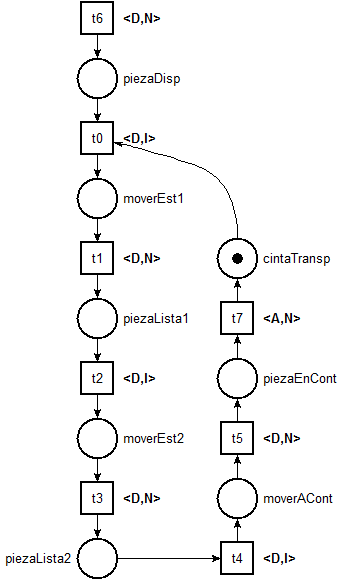
\includegraphics[height=100mm]{Petri_Cinta_Transportadora_2}
    \caption{Red de Petri de una cinta transportadora sincronizada por inserción
    de plaza-transición}
    \label{fig:petri_cinta_transportadora_2}
\end{figure}


Donde:\\
\begin{enumerate}
	\item Se generan eventos que se encolan en la cola de entrada en “t0, t2 y
		t4”.
	\item El monitor duerme los hilos que generaron eventos para “t0, t2 y t4” por
		no estar sensibilizadas las transiciones en ese momento.
	\item Llega una pieza y se genera un evento de entrada en “t6”
	\item El monitor dispara “t6” y se coloca un token en “piezaDisp”,
		sensibilizando “t0”.
	\item El monitor despierta el hilo dormido en “t0” ya que ahora tiene permiso
		de ejecución.
	\item Se ejecuta “moverEst1”. Una vez finalizado se genera un evento que se
		envía a la cola de entrada de “t1”.
	\item Como “t1” está sensibilizada el monitor la dispara y se coloca un token
		en “piezaLista1”, sensibilizando “t2”.
	\item El monitor despierta el hilo dormido en “t2” ya que ahora tiene permiso
		de ejecución.
	\item Se ejecuta “moverEst2”. Una vez finalizado se genera un evento que se
		envía a la cola de entrada de “t3”.
	\item Como “t3” está sensibilizada el monitor la dispara y se coloca un token
		en “piezaLista2”, sensibilizando “t4”.
	\item El monitor despierta el hilo dormido en “t4” ya que ahora tiene permiso
		de ejecución.
	\item Se ejecuta “moverACont”. Una vez finalizado se genera un evento que se
		envía a la cola de entrada de “t5”
	\item Como “t5” está sensibilizada el monitor la dispara y se coloca un token
		en ``piezaEnCont''.
	\item Se ejecuta la transición ``t7'', que es automática, y se libera el
		recurso ``cintaTransp''.
\end{enumerate}
La principal ventaja de este método es que no modifica la semántica de la red y
no añade nuevos conceptos ni cambios en su forma de ejecución.
La desventaja más importante es que puede provocar un incremento considerable de
la cantidad de plazas y transiciones de la red, lo que conlleva el
procesamiento de matrices de mayor tamaño.

\subsubsection{Sincronización por Guardas}
Este método consiste en la utilización de una guarda como forma de
sincronización entre tareas consecutivas. Ver Figura ~\ref{fig:petri_cinta_transportadora_3}

\begin{figure}[H]
    \centering
    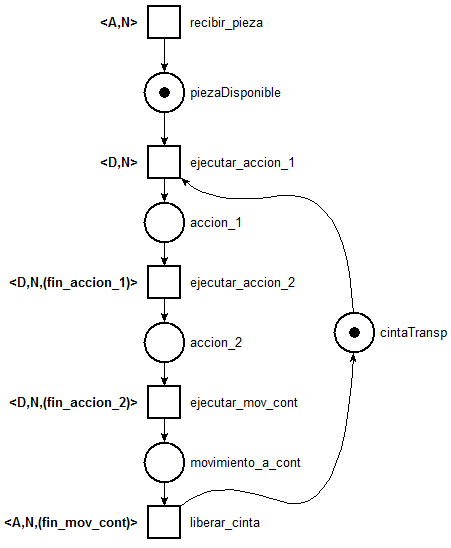
\includegraphics[height=100mm]{Petri_Cinta_Transportadora_3}
    \caption{Red de Petri de una cinta transportadora sincronizada por guardas.}
    \label{fig:petri_cinta_transportadora_3}
\end{figure}

\begin{enumerate}
    \item Se generan eventos que se encolan en la cola de entrada en “t0, t1 y
    t2”.
	\item El monitor duerme los hilos que generaron eventos para “t1 y t2” por
	no estar sensibilizadas las transiciones en ese momento.
	\item Se dispara ``t0'' y se coloca un token en ``moverEst1''. Comienza la
	ejecución de la tarea ``moverEst1''. La transición ``t1'' no se encuentra
	sensibilizada dado que la guarda ``Fin\_moverEst1'' tiene estado ``false''.
	\item Finaliza la ejecución de ``moverEst1'' y se setea la guarda
	``Fin\_moverEst1'' con estado ``true''.
	\item Al estar sensibilizada ``t1'', se dispara y se despierta el hilo que
	duerme en su cola de condición. Se coloca un token en ``moverEst2'' y
	comienza la ejecución de esta tarea. La transición ``t2'' no se
	encuentra sensibilizada dado que la guarda ``Fin\_moverEst2'' tiene estado
	``false''. Debe setearse la guarda ``Fin\_moverEst1'' a ``false'' nuevamente.
	\item Finaliza la ejecución de ``moverEst2'' y se setea la guarda
	``Fin\_moverEst2'' con estado ``true''.
	\item Al estar sensibilizada ``t2'', se dispara y se despierta el hilo que
	duerme en su cola de condición. Se coloca un token en ``moverACont'' y
	comienza la ejecución de esta tarea. La transición ``t3'' no se
	encuentra sensibilizada dado que la guarda ``Fin\_moverACont'' tiene estado
	``false''. Debe setearse la guarda ``Fin\_moverEst2'' a ``false'' nuevamente.
	\item Finaliza la ejecución de ``moverACont'' y se setea la guarda
	``Fin\_moverACont'' con estado ``true''.
	\item Al estar sensibilidada, se dispara la transición ``t3'', que es
	automática, y se libera el recurso ``cintaTransp''. Debe setearse la guarda
	``Fin\_moverACont'' a ``false'' nuevamente.
\end{enumerate}

La ventaja de este método es que permite resolver el problema de sincronización
sin aumentar la cantidad de componentes de la red de Petri.
Como desventaja se puede mencionar que la utilización de guardas modifica la
semántica de la red, complicando su demostración matemática. Además, el diseño del monitor de
petri soporta una única guarda por transición, por lo tanto esta solución impide
la utilización de la guarda para otros propósitos en una situación de tareas
consecutivas. Por último, otra desventaja importante de la utilización de
guardas es que al ser un valor binario no se puede saber cuantas veces ha sido seteada
la guarda.
Se supone un caso donde una ``tarea A'' es realizada por multiples hilos de manera
independiente, y cada hilo realiza la ``tarea A'' en su totalidad. A su
vez una ``tarea B'', que debe realizarse luego de la finalización de la ``tarea
A'', es ejecutada por un único hilo. En este caso la utilización de guardas
podría llevar a una pérdida de eventos de finalización de la ``tarea A'' debido
a la condición binaria de la guarda. Ver Figura ~\ref{fig:ejecucion_multiples_hilos_guardas}

\begin{figure}[H]
    \centering
    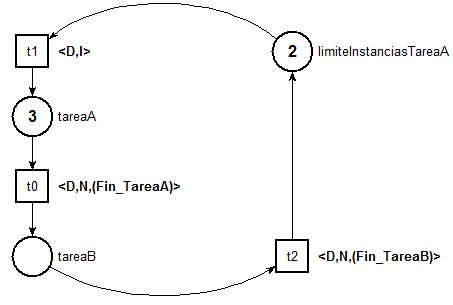
\includegraphics[height=60mm]{Ejecucion_Tarea_Multiples_Hilos_Guardas}
    \caption{RdP: Problema de sincronización de tareas sincrónicas usando
    guardas debido a su condición binaria}
    \label{fig:ejecucion_multiples_hilos_guardas}
\end{figure}

En esta red, un máximo de 5 hilos puede ejecutar la ``tarea A'' al mismo
tiempo. En el estado que  muestra la Figura
~\ref{fig:ejecucion_multiples_hilos_guardas} existen tres hilos corriendo la
``tarea A''. De acuerdo a lo supuesto en el planteo de este problema, la ``tarea
B'' es ejecutada por un único hilo. Si dos o más hilos finalizan la ``tarea A''
y setean la guarda ``Fin\_TareaA'' entonces, cuando se dispare ``t1" y antes de
comenzar la ejecución de la ``tareaB'', se debe modificar el valor de la guarda
``Fin\_TareaA'' a ``false'', y de esta manera existe la posibilidad de perder
eventos de finalización de la ``tarea A''.

\subsubsection{Sincronización por Disparo No Perenne de Aviso de
Finalización de Tarea}
Esta forma de solucionar la sincronización de tareas sincrónicas consecutivas
supone añadir una nueva propiedad ``P'' a las transiciones. Los hilos que
duermen en la cola de condición de una transición con propiedad ``P'' sólo
se despiertan cuando la transición se encuentra habilitada y además un hilo
externo realiza un disparo no perenne sobre la transición.

\begin{figure}[H]
    \centering
    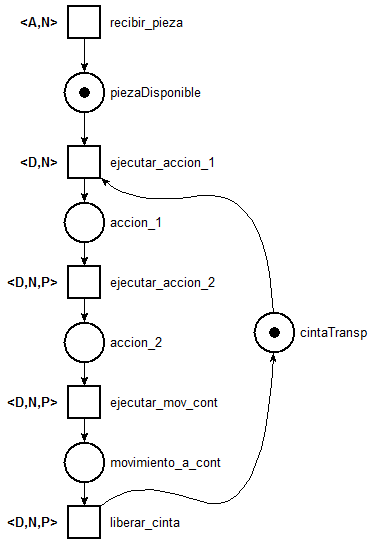
\includegraphics[height=100mm]{Petri_Cinta_Transportadora_4}
    \caption{Red de Petri de una cinta transportadora sincronizada por
    propiedad ``P''.}
    \label{fig:petri_cinta_transportadora_4}
\end{figure}

\begin{enumerate}
    \item Se generan eventos que se encolan en la cola de entrada en “t0, t1,
    t2 y t3”.
	\item El monitor duerme los hilos que generaron eventos para “t1, t2 y t3” por
	no estar sensibilizadas las transiciones en ese momento.
	\item Se dispara ``t0'' y se coloca un token en ``moverEst1''. Comienza la
	ejecución de la tarea ``moverEst1''. La transición ``t1'' no se dispara ya que
	es de tipo ``P'' y solo puede dispararse de forma no perenne por un hilo
	externo.
	\item Finaliza la ejecución de ``moverEst1'' y un hilo dispara ``t1'' de forma
	no perenne para dar aviso de la finalización de la tarea.
	\item Se despierta el hilo que
	duerme en cola de condición de ``t1''. Se coloca un token en ``moverEst2'' y
	comienza la ejecución de esta tarea. La transición ``t2'' no se dispara ya que
	es de tipo ``P'' y solo puede dispararse de forma no perenne por un hilo
	externo.
	\item Finaliza la ejecución de ``moverEst2'' y un hilo dispara ``t2'' de forma
	no perenne para dar aviso de la finalización de la tarea.
	\item  Se despierta el hilo que
	duerme en cola de condición de ``t2''. Se coloca un token en ``moverACont'' y
	comienza la ejecución de esta tarea. La transición ``t3'' no se dispara ya que
	es de tipo ``P'' y solo puede dispararse de forma no perenne por un hilo
	externo.
	\item Finaliza la ejecución de ``moverACont'' y un hilo dispara ``t3'' de forma
	no perenne para dar aviso de la finalización de la tarea.
	\item Se libera el recurso ``cintaTransp''.
\end{enumerate}

Esta solución tiene como principal ventaja mantener la cantidad de componentes
de la red de Petri.
Su principal desventaja consiste en que añade una nueva etiqueta a la
petri, dificultando su demostración matemática. Esta solución supone añadir una
interfaz al monitor de petri para dormir hilos en una cola de condición de una
transición tipo P y que los hilos bloqueados en esta cola de condición sólo
puedan liberarse por medio de un disparo no perenne ocasionado por un hilo
externo.
El hilo que realiza el disparo sobre la transición debe realizar una operación
release sobre la cola de condición de disparos no perennes (sin importar si
existen o no hilos bloqueados en la cola) para evitar la pérdida de eventos de
finalización de tarea.

\subsubsection{Resumen}
\label{sec:resumen_sincronizacion}
Existen dos maneras de coordinar la ejecución de las tareas a partir de una red
de Petri.\\ 
La primera consiste en suscribir una tarea a una transición y que se
informe a la tarea cuando la transición es disparada. En caso de ser
una tarea sincrónica, se dispara otra transición al finalizar la misma. Esta
transición disparada tendrá suscripta la siguiente tarea a ejecutar e informará
su disparo a dicha tarea. Este modo de ejecución tiene una desventaja
importante que consiste en la descentralización del manejo de los hilos por
parte del monitor, atribuyendole al manejador de eventos y al manejador de
acciones parte de la responsabilidad de esta tarea. Al delegar el manejo del
informe de una transición informada, se delega la responsabilidad de
despertar o crear el hilo que ejecute la tarea suscripta a dicha transición. De
esta forma se desaprovecha una de las principales ventajas de la arquitectura
de un sistema con monitor.\\
El segundo modo consiste en hilos pidiendo permiso de ejecución al monitor
mediante el disparo de las transiciones correspondientes a las tareas que deben
realizar. De esta forma el monitor duerme los hilos que no pueden ejecutarse y
despierta aquel hilo que duerma en la cola de condicion de la
transición que se dispara. De esta forma el manejo de la concurrencia y de los
hilos es llevado a cabo íntegramente por el monitor. Sin embargo, para
sincronizar tareas dependientes entre sí (una debe comenzar luego de la
finalización de la otra) debe existir una forma de dar aviso al monitor de la
finalización de una tarea. En este trabajo se adopta esta forma de
sincronicación por petición de ejecución.\\
En esta sección se analizaron tres formas de realizar el aviso de finalización
de tareas en un modo de ejecución por petición, Por transición-plaza, por
guardas y por transiciones tipo ``P''.\\
 Tras analizar estos tres modelos de redes de Petri se decidió optar por añadir
 un conjunto transición-plaza como forma de sincronización. Si bien presenta la
 desventaja de incrementar el número de plazas y transiciones de la red, con su
 inherente incremento de tamaño de matrices a procesar, permite utilizar una
 ejecución guiada por permiso de ejecución (centralizando el control de flujo
 de ejecución en el monitor). Además no añade conceptos nuevos a la red,
 facilitando el entendimiento de la misma.
 
 
 
 
 
